\begin{anexosenv}

\partanexos

\chapter{Telas do \textit{software} Pé na Estrada}
  
  \section{Tela de ranking das rodovias federais}
    \begin{figure}[!htb]
      \centering
      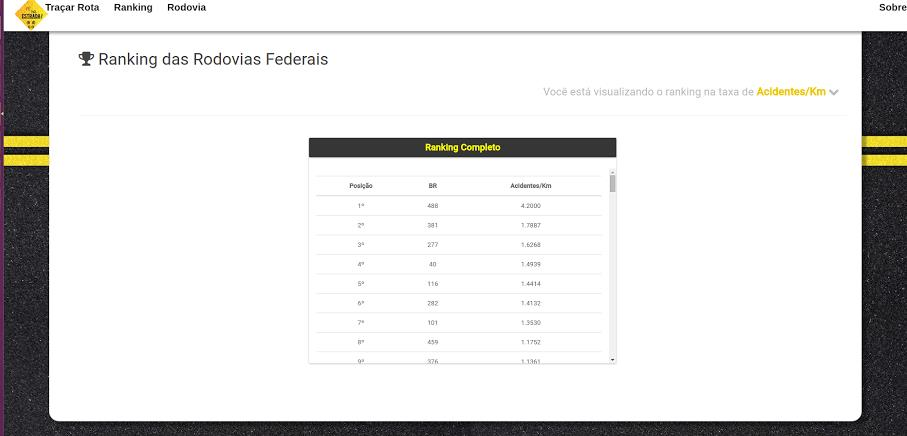
\includegraphics[scale = 0.5, angle=90]{ranking_penaestrada}
      \caption[Tela de ranking das rodovias federais]{Tela de ranking das rodovias federais.}
      \label{fig:ranking_penaestrada}
    \end{figure}
    
    \vfill
  
  \pagebreak
  \section{Tela de sinalização dos acidentes em uma rota}
    \begin{figure}[!htb]
      \centering
      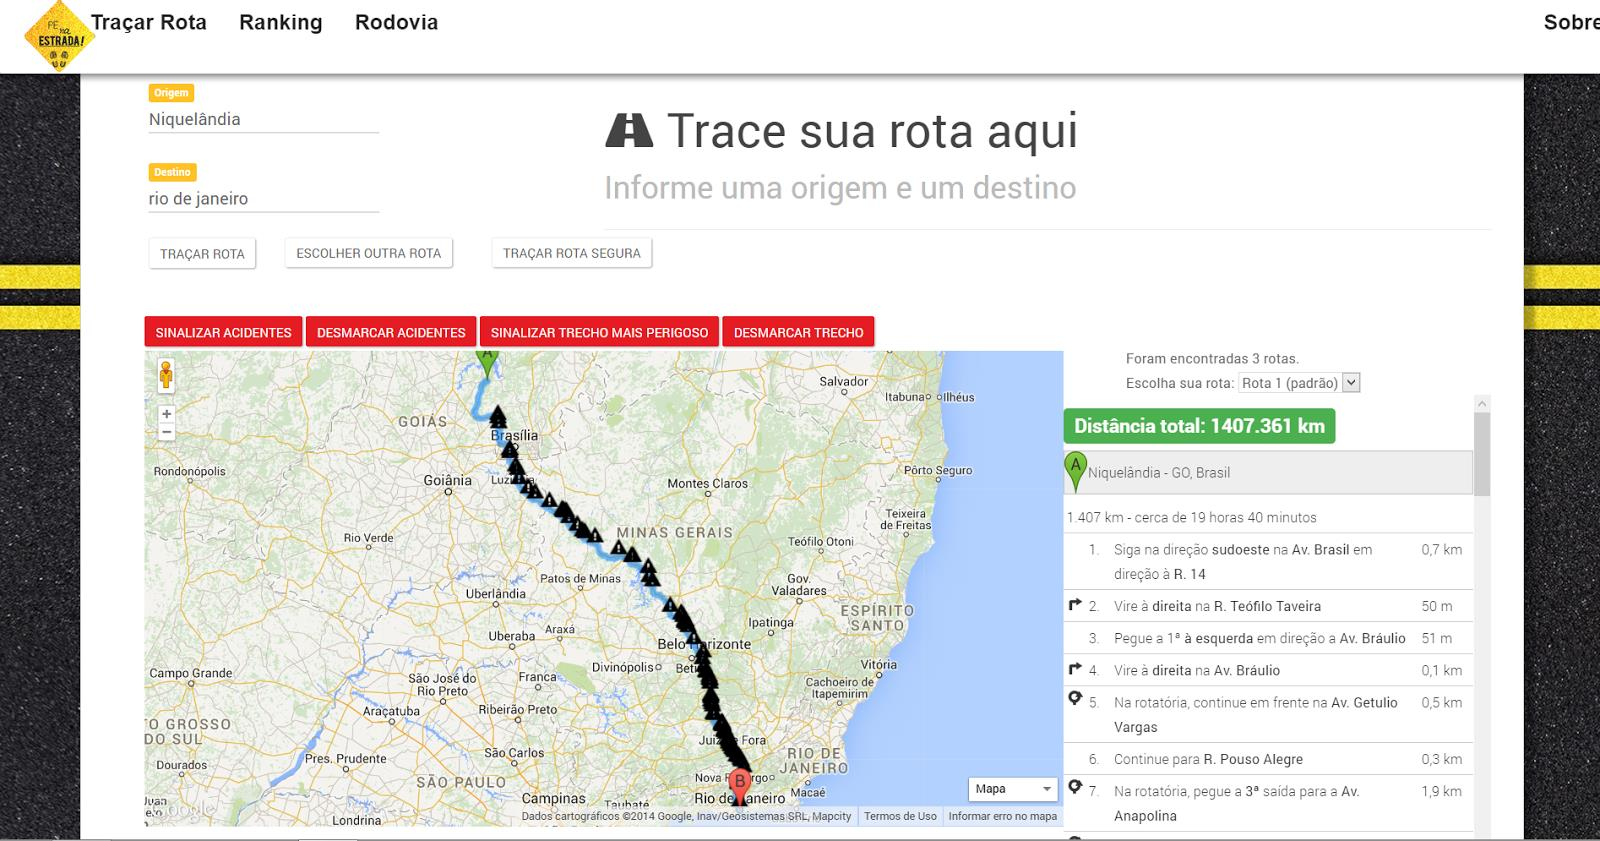
\includegraphics[scale = 0.35, angle=90]{rota_penaestrada}
      \caption[Tela de sinalização dos acidentes em uma rota]{Tela de sinalização dos acidentes em uma rota.}
      \label{fig:rota_penaestrada}
    \end{figure}
    
    \vfill
    
  \pagebreak
  \section{Tela de sinalização do trecho mais perigoso de uma rota}
  
    \begin{figure}[!htb]
      \centering
      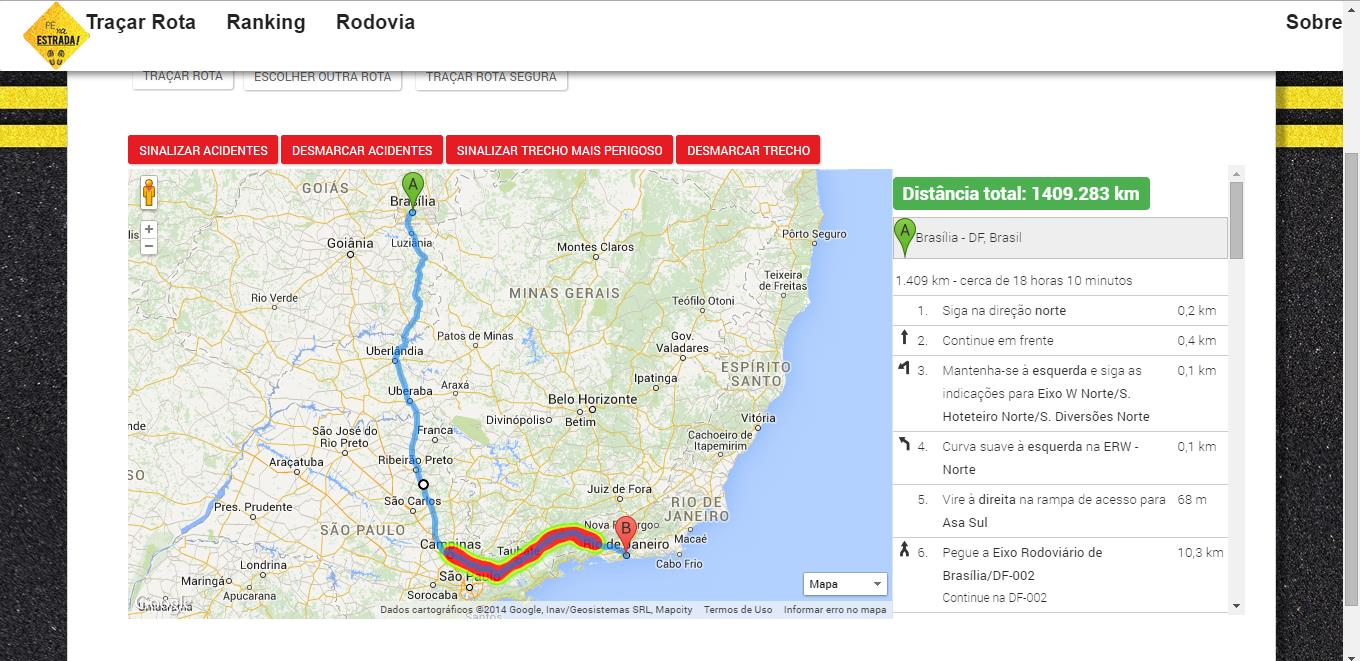
\includegraphics[scale = 0.4, angle=90]{trecho_penaestrada}
      \caption[Tela de sinalização do trecho mais perigoso de uma rota]{Tela de sinalização do trecho mais perigoso de uma rota.}
      \label{fig:trecho_penaestrada}
    \end{figure}
    
    \vfill
    
\end{anexosenv}

